\documentclass[letterpaper]{article}

%% Language and font encodings
\usepackage[english]{babel}
\usepackage[utf8]{inputenc}
\usepackage[pdftex]{graphicx}

\newcommand{\timeline}{\hspace{-2.3pt}$\bullet$ \hspace{5pt}}

\usepackage{booktabs}
\usepackage{tabu}
\usepackage[T1]{fontenc}
\usepackage[backend=biber, style=ieee]{biblatex}
\addbibresource{prop.bib}

%% Sets page size and margins
\usepackage[a4paper,top=3cm,bottom=2cm,left=3cm,right=3cm,marginparwidth=1.75cm]{geometry}

%% Useful packages
\usepackage{amsmath}
\usepackage{graphicx}
%\usepackage{apacite}
\usepackage[colorinlistoftodos]{todonotes}
\usepackage[colorlinks=true, allcolors=blue]{hyperref}

\title{Product Quality Prediction in Laser-Induced Forward Transfer (LIFT) Process using Machine Learning}
\author{Team 13 \\ Md Shahriar Forhad\\Amit Das\\Alfredo J. Pena\\ \\Supervisor\\Dr. Dongchul Kim}
\date{September 10th, 2021}

\begin{document}
\maketitle

\section*{Summary of the Proposal}
Additive manufacturing plays a key role in the printed electronics field, which is used in a wide variety of applications, such as diverse types of sensors, solar cells etc. Colloidal ink is used to print electronic circuits by Laser-Induced Forward Transfer (LIFT) process. Finding out optimal laser parameters requires a lot of work, which is time-consuming and costly. In recent years, Machine Learning (ML) has gained interest among researchers to be employed in manufacturing industries to optimize process parameters and predict product quality. Our goal is to develop an ML model to predict the product quality in accordance with the input parameters and find out the significance of different parameters using the Principal Component Analysis (PCA). Besides, pictures will be taken during the experiment to classify the quality. The experimental data will be collected from the Industrial and Manufacturing Engineering Department of the University of Texas at Rio Grande Valley.

\section*{Background}
The unparalleled computing capabilities of Artificial Intelligence (AI) and machine learning (ML) have introduced new dimensions in every science and technology field. These data hungry AI models need a large amount of data as input to give state-of-the art output, and increasing data generation and storing capabilities make this possible. The current scenario of interdisciplinary research unveils new possibilities, from medical to management, in every research field, so as in Additive Manufacturing (AM).
\par
Laser-induced forward transfer (LIFT) utilizes pulsed laser that is incident on a thin film of a precursor ink in order to transferring the droplets of the ink onto a receiver substrate \parencite[]{pradas}. Not requiring any lithographic process makes LIFT process so intelligible and a very important tool for prototyping or repair \parencite[]{arnold}. So, LIFT process is achieving interest among the researchers as a printing technology for gas sensors, photovoltaic cells, and printed electronics. Machine learning can play a vital role in situ monitoring and control which is a very important component of Industry 4.0.
\par
Monitoring and control of a LIFT process is challenging because materials are liquefied and solidified within picoseconds. High-speed camera, especially IR camera helps us a lot to learn more about the melting and solidification process. Machine Learning can help us to classify different states, so that it will be easier for us to find out causes of different faults or diversity in output.
\par
In Additive Manufacturing, machine learning models are used in various ways, e.g., defect detection, control, and prediction. These pre-inspections increase the efficiency of the traditional manufacturing process and cost-effective in many folds. For Instance, A CNN was used in AM to make the production robust, less biased- and this algorithm was able to detect manufacturing parts with 92.4\% accuracy \parencite[]{cui}. In this way, scholars have underscored the power of AI in various ways to mitigate preprocessing costs and bolster their research.
\par
\begin{figure}[h!]
  \centering
  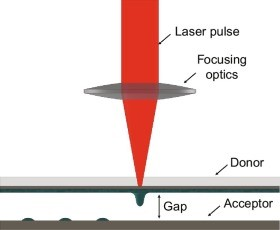
\includegraphics[width=175pt]{images/fig1.jpg}
  \caption{Standard LIFT Process \parencite[]{morales}}
  \label{fig:stdlift}
\end{figure}

\section*{Goal and Objectives}
The goal is to reduce number of experiment required to get required quality product in a LIFT system. The objective is to develop a machine learning model to reduce the cost and time required for that kind of experiment. Machine learning will aid reduce cost by decreasing the number of experiment required and with less time the researchers may be able to establish the process parameters to achieve the product with expected attributes.

\section*{Data and Methods}
ML is gaining interest among the researchers to be employed in different area like study in thermodynamics \parencite[]{ding}, \parencite[]{thermal},  High-Entropy Alloys (HEAs)\parencite[]{qiao}, material staleness's \parencite[]{he}, etc. Many experiments have been conducted on LIFT process, but employing ML to predict the product quality has hardly been found to be implemented for that process.
\par
Nanoparticles will be synthesized using LIFT process where laser power, water level and irradiation time will be controlled to find out respective average particle size. These process parameters will be selected as per design of experiment theory (taguchi, factorial methods) to ensure proper variability in the input to ease to develop a relation between the input and output parameters using machine learning. Since, the experiments are time-consuming and costly, with fewer samples how to build a good ML model will be a challenge and different methods will be employed (regression, neural network) with different hyperparameters to find out a dependable ML model. Besides, video/pictures will be captured during the process and these pictures will be analyzed using unsupervised learning to find out whether we can classify the quality from the pictures. Later, this will be helpful to develop \textit{in situ} monitoring of the LIFT process.\par
Process are made smarter with AI, that has a wide range of application like management, auto-identification and maintenance \parencite[]{xu}. \parencite[]{bourhis}. Considered Machine learning to be able to substitute field-testing in a wide range. Recently researchers are trying to utilize machine learning in almost every sector, for example in medical sectors \parencite[]{twin}, aeronautical manufacturing industries \parencite[]{zohdi}, climate prediction \parencite[]{koc}.  Furthermore, \parencite[]{tapia}  studied predictive model for additive manufacturing and \parencite[]{kharchenko} worked on AI-assisted decision support system.
\par
We will construct a novel data set from the IME lab experiments, by using the data set we will use various image analysis models, such as- Multivariate Image Analysis (MIA), and Multivariate Image Regression (MIR) for prediction \parencite[]{duchesne}, finally, providing a case study models of using classifiers for the quality control of laser-Induced additive manufacturing.

\section*{Timeline}

\scalebox{1}{
\begin{tabular}{r |@{\timeline} l}

Week- 1 Sep'21 & Brain storming and literature Review about the Project\\
\\
Week- 2 & Started Writing the proposal and submission\\
\\
Week-3 \& 4 & Gathering  Data from the Experiment(IME LAB UTRGV)\\
\\
Week-1 Oct'21 & Start running models on the generated data \\&for aiding the lab experiments\\
\\
Week 2-4 & Finding the accuracy of our predictions \\ & by comparing with the real-lab experiments\\
\\
3 Weeks Before Submission & Final Presentation\\
\\
 Last week of Fall'21 &  Complete project report submission\\

\end{tabular}
}

\printbibliography



\end{document}